% Copyright 2004 by Till Tantau <tantau@users.sourceforge.net>.
%
% In principle, this file can be redistributed and/or modified under
% the terms of the GNU Public License, version 2.
%
% However, this file is supposed to be a template to be modified
% for your own needs. For this reason, if you use this file as a
% template and not specifically distribute it as part of a another
% package/program, I grant the extra permission to freely copy and
% modify this file as you see fit and even to delete this copyright
% notice. 

\documentclass{beamer}

% There are many different themes available for Beamer. A comprehensive
% list with examples is given here:
% http://deic.uab.es/~iblanes/beamer_gallery/index_by_theme.html
% You can uncomment the themes below if you would like to use a different
% one:
%\usetheme{AnnArbor}
%\usetheme{Antibes}
%\usetheme{Bergen}
%\usetheme{Berkeley}
%\usetheme{Berlin}
%\usetheme{Boadilla}
%\usetheme{boxes}
%\usetheme{CambridgeUS}
%\usetheme{Copenhagen}
%\usetheme{Darmstadt}
\usetheme{Edinburgh}
%\usetheme{Frankfurt}
%\usetheme{Goettingen}
%\usetheme{Hannover}
%\usetheme{Ilmenau}
%\usetheme{JuanLesPins}
%\usetheme{Luebeck}
%\usetheme{Madrid}
%\usetheme{Malmoe}
%\usetheme{Marburg}
%\usetheme{Montpellier}
%\usetheme{PaloAlto}
%\usetheme{Pittsburgh}
%\usetheme{Rochester}
%\usetheme{Singapore}
%\usetheme{Szeged}
%\usetheme{Warsaw}

\title{mappED}

% A subtitle is optional and this may be deleted
%\subtitle{Optional Subtitle}

\author{Thomas Kozlowski \\
Andrew Lindsay \\
Jaka Mohorko \\
Alexander Pietz}

\date{Smart Data Hack 2016}
% - Either use conference name or its abbreviation.
% - Not really informative to the audience, more for people (including
%   yourself) who are reading the slides online

\subject{Theoretical Computer Science}
% This is only inserted into the PDF information catalog. Can be left
% out. 

% If you have a file called "university-logo-filename.xxx", where xxx
% is a graphic format that can be processed by latex or pdflatex,
% resp., then you can add a logo as follows:

\pgfdeclareimage[height=1.5cm]{university-logo}{EdinburghUniLogo}
 \logo{\pgfuseimage{university-logo}}

% Delete this, if you do not want the table of contents to pop up at
% the beginning of each subsection:
\AtBeginSubsection[]
{
  \begin{frame}<beamer>{Outline}
    \tableofcontents[currentsection,currentsubsection]
  \end{frame}
}

% Let's get started
\begin{document}

\begin{frame}
  \titlepage
\end{frame}

\begin{frame}{Outline}
  \tableofcontents
  % You might wish to add the option [pausesections]
\end{frame}

% Section and subsections will appear in the presentation overview
% and table of contents.
\section{The Problem}


\begin{frame}{Finding a building}{(And a room)}
  \begin{itemize}
  \item {
    Have you ever looked at you exam timetable just to find that the location looks a little something like this?
  }\pause
  \item {
    "James Clerk Maxwell Building - Room 5327"
  }
  \end{itemize}
\end{frame}

%\subsection{Second Subsection}
\subsection{Finding a Building}
% You can reveal the parts of a slide one at a time
% with the \pause command:
\begin{frame}{Finding a Building}{Campus Map}
  \centerline{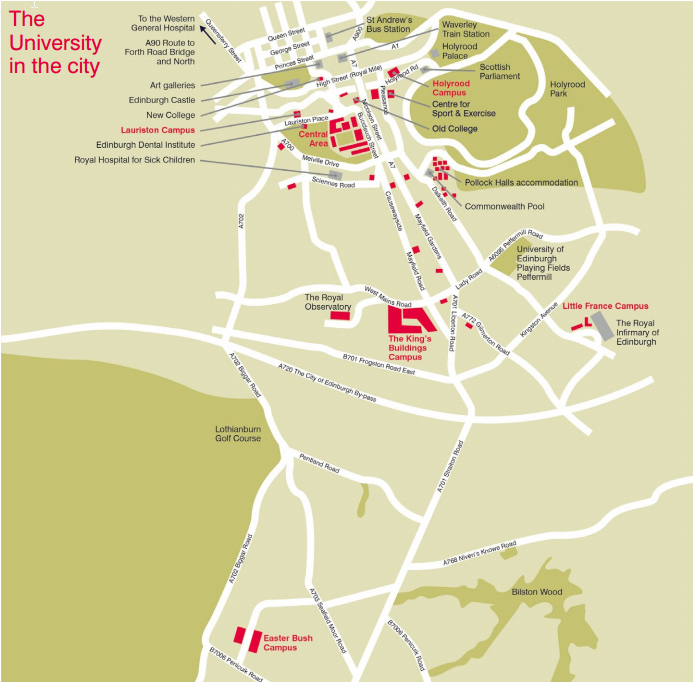
\includegraphics[height=0.8\textheight]{campusmap.png}}
\end{frame}

\begin{frame}{Finding a Building}{A-Z List}
  \centerline{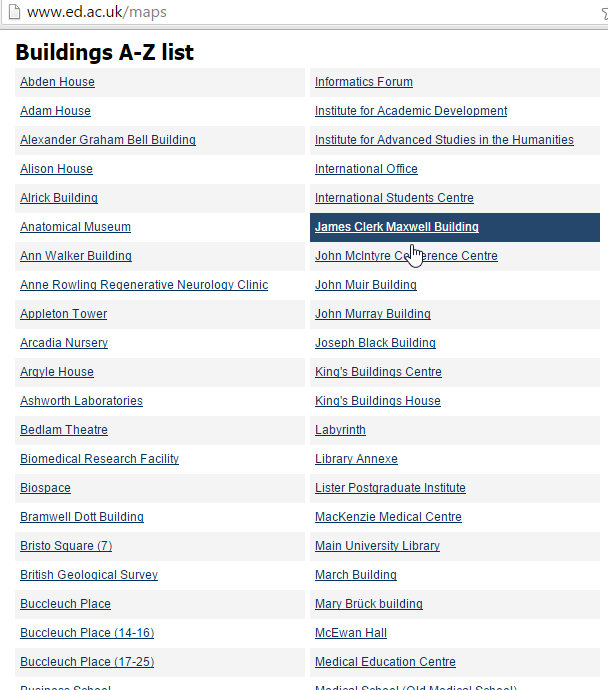
\includegraphics[height=0.8\textheight]{atozlist.png}}
\end{frame}

\begin{frame}{Finding a Building}{A-Z List - Map}
  \centerline{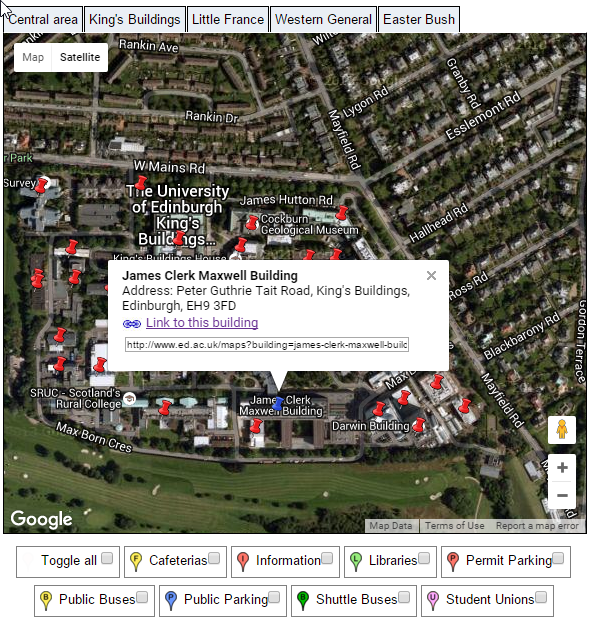
\includegraphics[height=0.8\textheight]{atozmap.png}}
\end{frame}
\subsection{Finding a Room}
\begin{frame}{Finding a Room}{Looking for the floorplan}
  \centerline{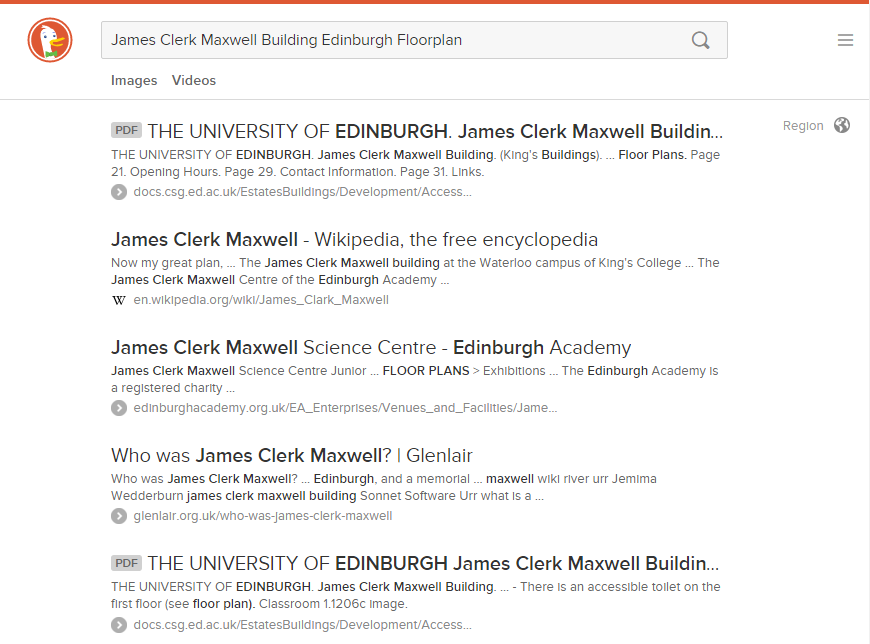
\includegraphics[height=0.8\textheight]{floorplansearch.png}}
\end{frame}

\begin{frame}{Finding a Room}{Navigating the floorplan}
  \centerline{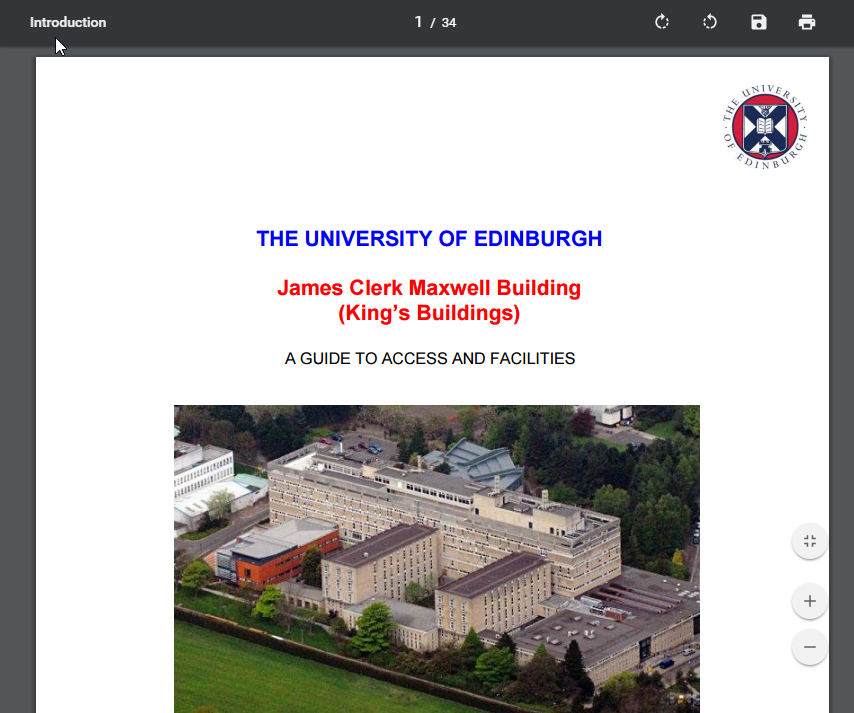
\includegraphics[height=0.8\textheight]{pdf1.png}}
\end{frame}

\begin{frame}{Finding a Room}{Navigating the floorplan}
  \centerline{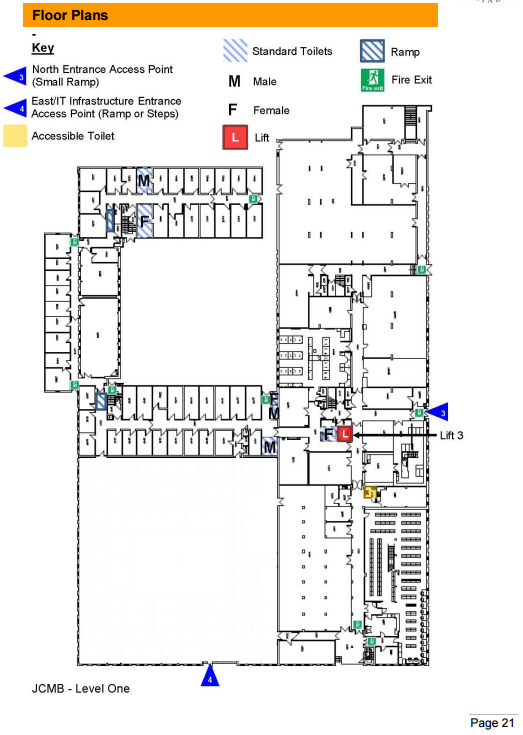
\includegraphics[height=0.8\textheight]{pdf2.png}}
\end{frame}

\begin{frame}{Finding a Room}{Navigating the floorplan}
  \centerline{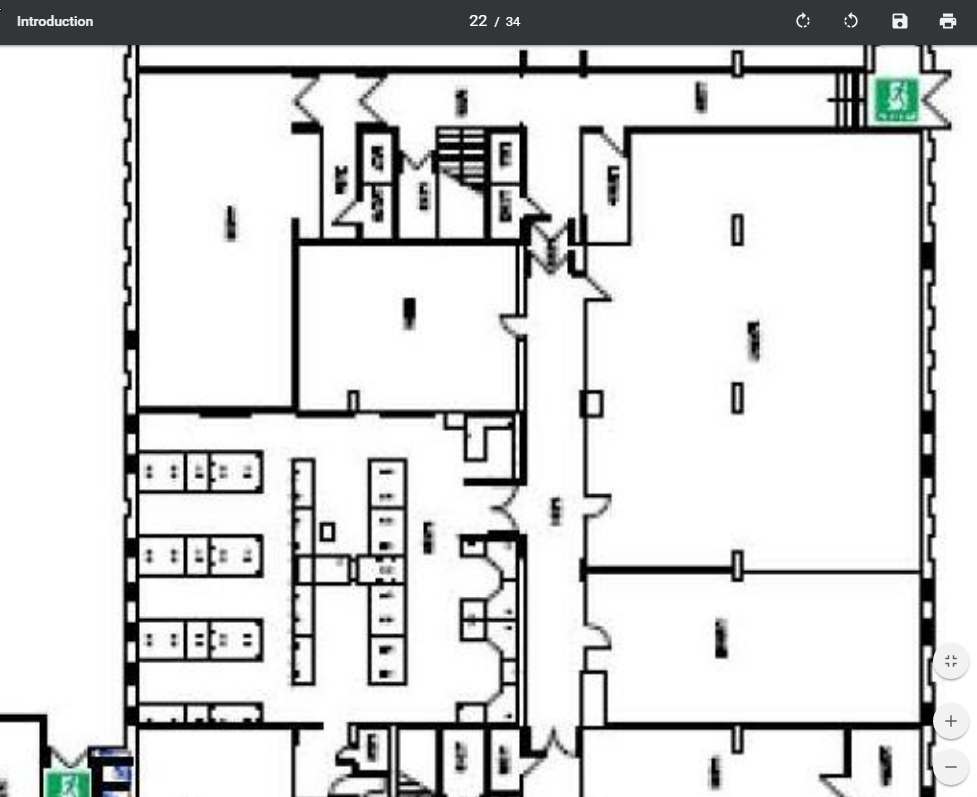
\includegraphics[height=0.8\textheight]{pdf3.png}}
\end{frame}

\section{The Solution}

\begin{frame}{Our Goal}
\begin{block}{Abstract}
There are several resources on locations at the University scattered all over the place - Finding a room inside a building that you have never been to can be quite the endeavour. We wanted to change this by creating one centralized place providing location and information on all University buildings, including things like Floorplans, Facilities, [..]
\end{block}
\end{frame}

% Placing a * after \section means it will not show in the
% outline or table of contents.
\section*{Summary}

\begin{frame}{Summary}
  \begin{itemize}
  \item
    The \alert{first main message} of your talk in one or two lines.
  \item
    The \alert{second main message} of your talk in one or two lines.
  \item
    Perhaps a \alert{third message}, but not more than that.
  \end{itemize}
  
  \begin{itemize}
  \item
    Outlook
    \begin{itemize}
    \item
      Something you haven't solved.
    \item
      Something else you haven't solved.
    \end{itemize}
  \end{itemize}
\end{frame}



% All of the following is optional and typically not needed. 
\appendix
\section<presentation>*{\appendixname}

\end{document}


